\section{Renormalization Group Flows}
\subsection{Review}
We studied how couplings ``flow'' upon integrating out a thin shell $b\Lambda < p < \Lambda$

\begin{center}
    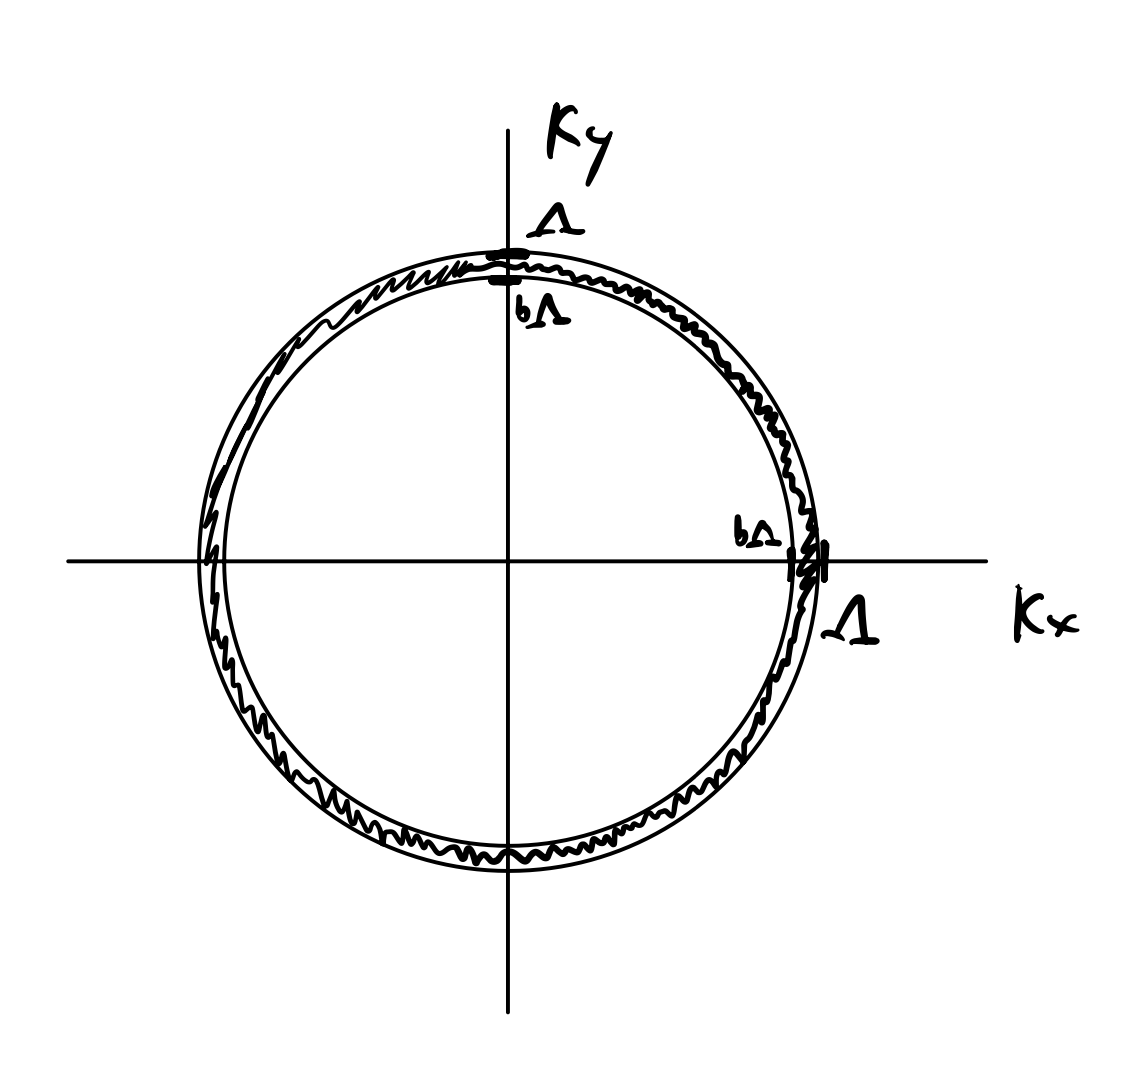
\includegraphics[scale=0.35]{Lectures/Figures/lec14-momentumshell.png}
\end{center}

(should be $p$ in the figure above, but I got lazy and did not want to redraw it). We considered the action:
\begin{equation}
    S = \int d^4x \frac{1}{2}(\nabla \phi)^2 + \frac{1}{2}m^2\phi^2 + \frac{\lambda}{4!}\phi^4
\end{equation}
upon integrating out the field, we had:
\begin{equation}
    Z = \int \mathcal{D}\phi e^{-S[\phi]}\int D\phi' e^{-S_{\text{int}}[\phi, \phi']}e^{-S[\phi']} = \int \mathcal{D}\phi e^{-S_{\text{eff}}[\phi]}
\end{equation}
Expanding in the interaction:
\begin{equation}
    Z = \int \mathcal{D}\phi \int \mathcal{D}\phi' (1 - S_{\text{int}} + \frac{1}{2}S_{\text{int}}^2 + ldots)e^{-S[\phi']}
\end{equation}
Where:
\begin{equation}
    S_{\text{int}} = \frac{\lambda}{4!}\int d^4x 4\phi^3\phi' + 6\phi^2\phi'^2 + 4\phi\phi'^3.
\end{equation}
Then to $O(\lambda)$:
\begin{equation}
    Z = \int \mathcal{D}\phi e^{-S[\phi]}\left(1 - \frac{\lambda}{4}\int d^4x \phi^2 \avg{\phi'^2(x)} + \ldots\right)
\end{equation}
where:
\begin{equation}
    \avg{\phi'^2(x)} = \frac{\Lambda^2}{(4\pi)^2}(1 - b^2)
\end{equation}
Thus:
\begin{equation}
    Z = \int \mathcal{D}\phi e^{-S[\phi]}\left(1 - \int \frac{1}{2}\Delta m^2 \phi^2\right)
\end{equation}
With:
\begin{equation}
    \Delta m^2 = \frac{\lambda\Lambda^2}{2(4\pi)^2}(1 - b^2).
\end{equation}
This contribution is pictorially depicted in the diagrams:

\begin{center}
    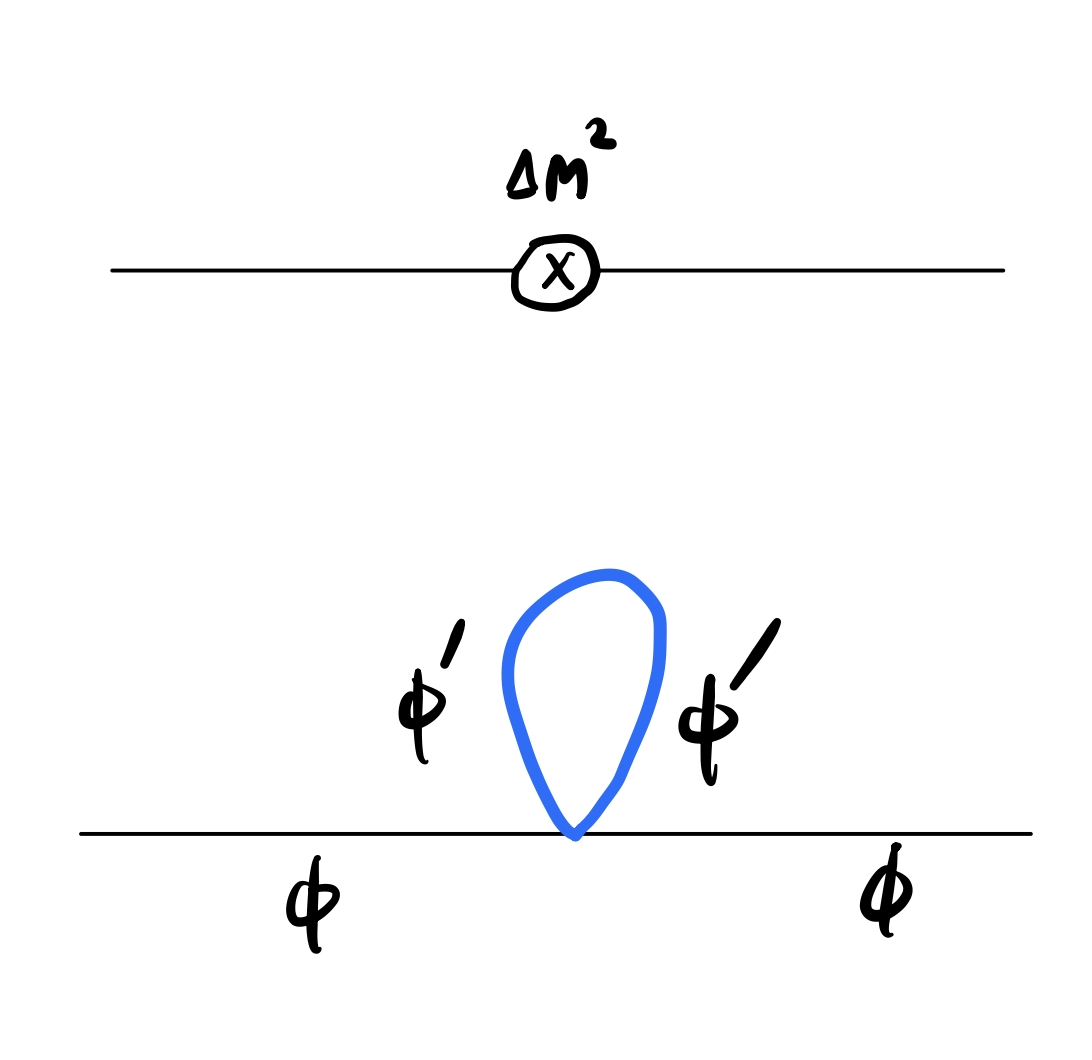
\includegraphics[scale=0.3]{Lectures/Figures/lec15-masscorrection.png}
\end{center}

This isn't so interesting, because the shift of the mass term is just a shift in the classical action. But the renormalization of the \emph{couplings} will be very interesting. This will be particularly interesting when we have theories with dimensionless couplings, when we can't use dimensional analysis to conclude that the coupling is relevant or irrelevant. The flow of the couplings will teach us this information.

\subsection{Renormalizing the interaction}
At higher orders, interactions renormalizes interactions; we have contributions from diagrams like:

\begin{center}
    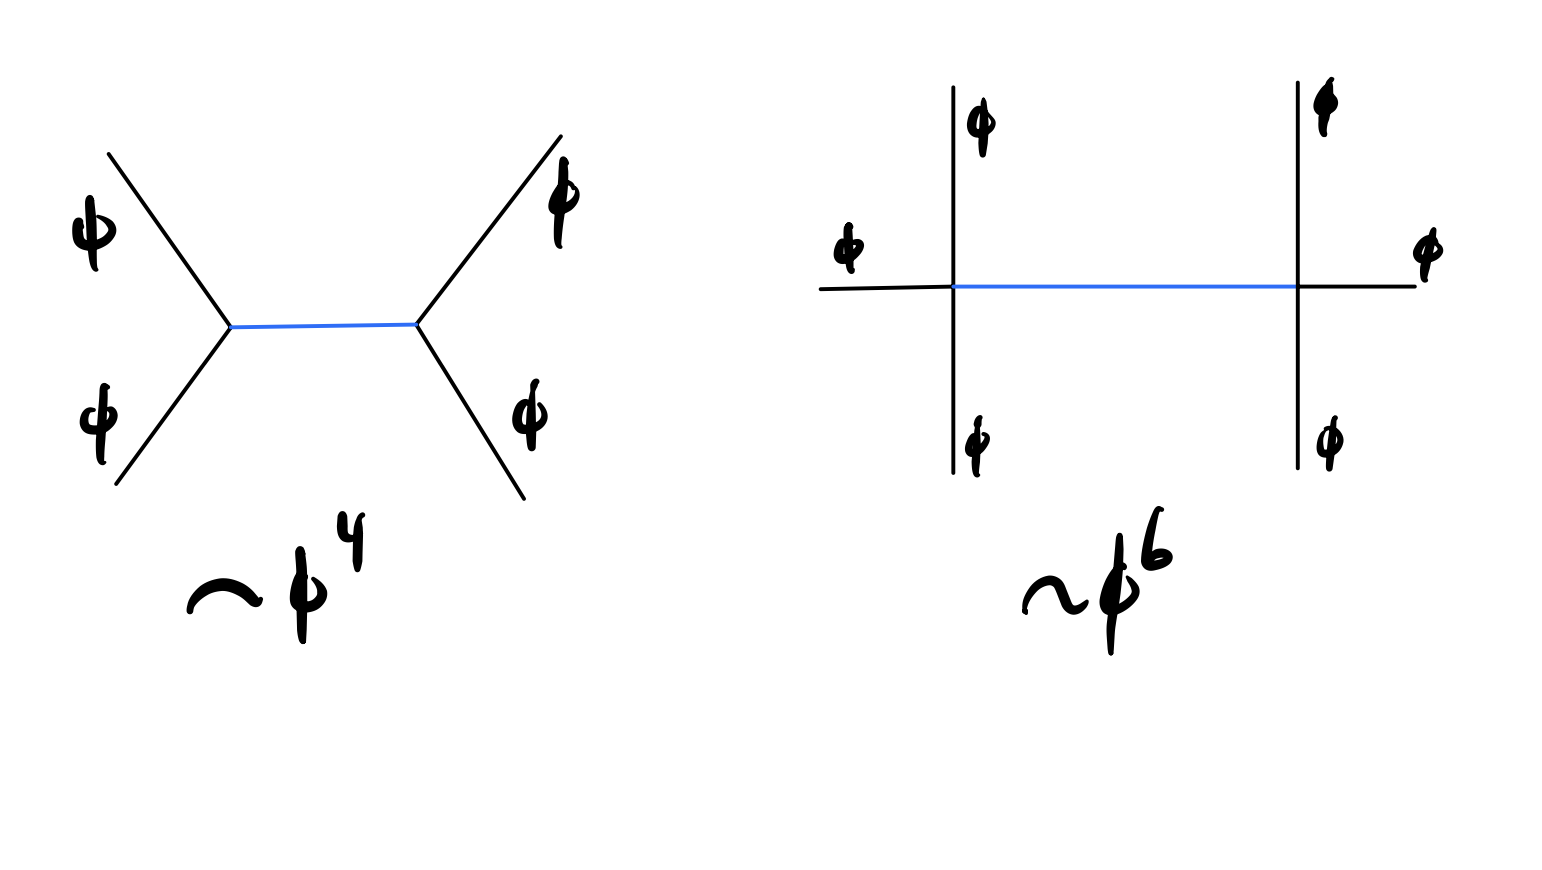
\includegraphics[scale=0.3]{Lectures/Figures/lec15-diagrams.png}
\end{center}

It is worth noting that at this order of $O(\lambda^2)$, several terms/diagrams contribute, but we focus on terms with 4 external fields, as these are the ones that will enter the renormalization of our interaction.

We look at:
\begin{equation}
    S_{\text{int}} = \frac{\lambda}{4}\int d^4x \phi^2(x)\phi'^2(x)
\end{equation}
What we are supposed to compute here is:
\begin{equation}
    Z = \int \mathcal{D}\phi e^{-S}\int \mathcal{D}\phi'\left(1 + S_{\text{int}} + \frac{1}{2}S_{\text{int}}^2 + \ldots \right)e^{-S[\phi']}
\end{equation}
we then need to compute:
\begin{equation}
    (A) = \frac{1}{2}\left(\frac{\lambda}{4}\right)^2\int d^4x d^4x' \phi^2(x)\phi^2(x')\avg{\phi'^2(x)\phi'^2(x')}.
\end{equation}

Where due to Wick contractions the four-point function appearing above just gives us a term $2G(x - x')^2$. This is a loop diagram, and its not too hard to compute. As usual, we work in momentum space:

\begin{center}
    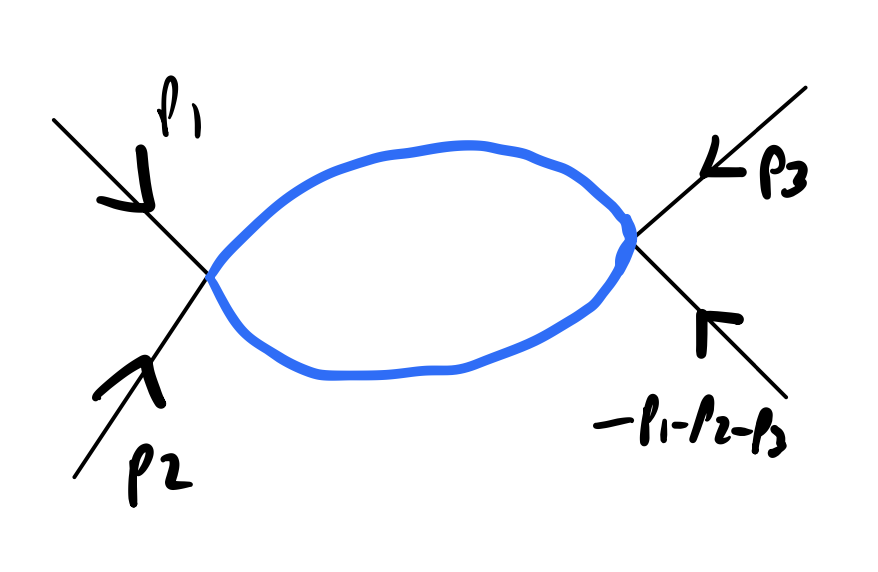
\includegraphics[scale=0.3]{Lectures/Figures/lec15-momentum.png}
\end{center}

so the term is:
\begin{equation}
    (A) = \left(\frac{\lambda}{4}\right)^2\int_{p_1p_2p_3}\phi_{p_1}\phi_{p_2}\phi_{p_3}\phi_{-p_1-p_2-p_3}\int_{p'}G(p')G(-p')
\end{equation}
Assuming $\Lambda \gg p_1, p_2, p_3$ and $\Lambda \gg m$, The $p'$ integral (only in the small shell near $\Lambda$) appearing above gives:
\begin{equation}
    \int_{p'}G(p')G(-p') = \int \frac{d^4p'}{(2\pi)^4}\frac{1}{(p')^4} = \frac{2\pi^2}{(2\pi)^4}\int_{b\Lambda}^\Lambda \frac{dp'}{p'} = \frac{1}{8\pi^2}\log \frac{1}{b}
\end{equation}
So Fourier transforming back, we obtain a correction which we interpret as a correction to the coupling:
\begin{equation}
    Z = \int \mathcal{D}\phi e^{-S[\phi]}\left(1 - \frac{\Delta \lambda}{4!}\int_x \phi^4(x) + \ldots\right)
\end{equation}
with:
\begin{equation}
    \Delta \lambda = -\frac{3\lambda^2}{(4\pi)^2}\log \frac{1}{b} < 0.
\end{equation}
Thus, we found that the effective coupling decreased. What this tells us is that as we go to lower and lower energies (as we coarse grain), the coupling becomes weaker and weaker. Thus, perturbation theory should become more controlled, and at very low energies the theory should become free. At tree level, studying the dimensions we concluded it was marginal. With our more careful analysis here, we found that the coupling is \emph{marginally irrelevant}. Examples of QFTs with marginally irrelevant couplings are:
\begin{itemize}
    \item $\phi^4$ theory in $D = 4$ or $D = 3 + 1$
    \item QED in $D = 4$
    \item Hydrodynamics in $D = 2 + 1$
\end{itemize}
A certain time ago, researchers thought that perhaps all theories were this way. However, this is not the case; examples of QFT with marginally relevant couplings are:
\begin{itemize}
    \item QCD in $D = 4$
    \item BCS theory of superconductivity in any dimension
    \item Non-linear $\sigma$ models in $D = 2$
\end{itemize}

Philosophical aside - RG tells us that we can't live in more than 4 dimensions, because in more than 4 dimensions we can't have dimensionless couplings (up to ongoing research). But for gravity we want $D \geq 4$. So $D = 4$ is the sweet spot.

\subsection{The $\beta$ function}
The $\beta$ function characterizes how the coupling changes with scale. Luca never remembers the sign convention, but it is defined as:
\begin{equation}
    \beta_\lambda = \dod{\lambda}{\log b}
\end{equation}
so for $\lambda \phi^4 > 0$ we have:
\begin{equation}
    \beta_\lambda = \frac{3\lambda^2}{(4\pi)^2} > 0.
\end{equation}
Thus we have that the coupling is marginally irrelevant if $\beta > 0$ and relevant if $\beta < 0$. In PS8, we will look at a case where the $\beta$ function vanishes due to competition of two terms. This is a situation where the theory is scale invariant, and corresponds to a RG fixed point.

\subsection{Callan-Symmezik Equation}
So - we learned how couplings can flow under coarse graining, but we still have the problem of the logarithmic corrections for marginal couplings. How can we use what we have learned to regain control of our perturbation expansion and make predictions for our observables? This brings us to the Callan-Symmezik equation. It is discussed in full generality in Peskin 12.3; here we study a simpler version.

The simplest thing we could use to probe the coupling is the four point function (we will see later that this can also be interpreted as a 2-to-2 scattering) $\avg{\phi_{p_1}\phi_{p_2}\phi_{p_3}\phi_{-p_1-p_2-p_3}}$:

\begin{center}
    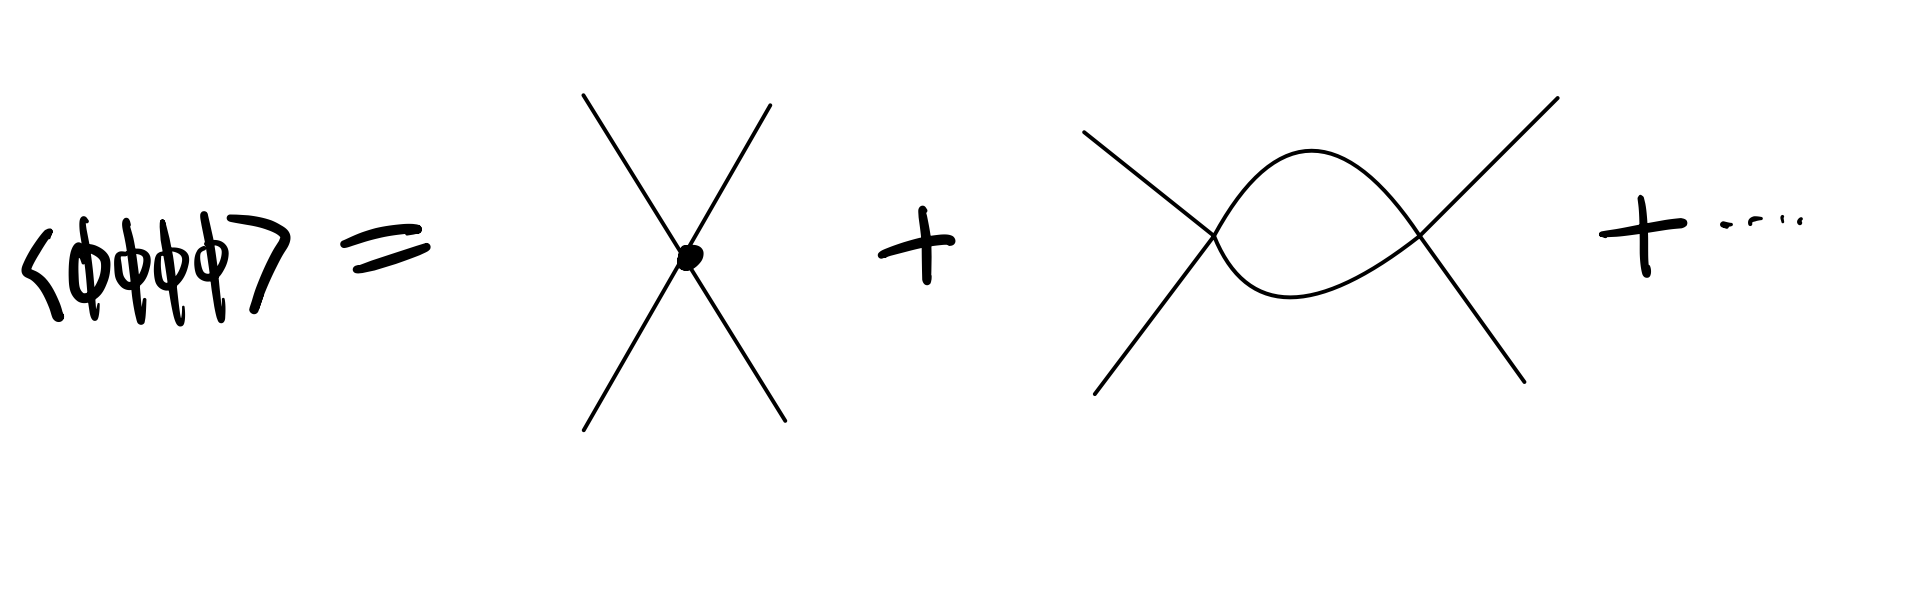
\includegraphics[scale=0.3]{Lectures/Figures/lec15-phi4observable.png}
\end{center}

Which evaluates to:
\begin{equation}
    \avg{\phi_{p_1}\phi_{p_2}\phi_{p_3}\phi_{-p_1-p_2-p_3}} = G(p_1)G(p_2)G(p_3)G(-p_1-p_2-p_3)\left[-\lambda + \left(\frac{\lambda}{4}\right)^2\int_{p'}G(p')G(p_1 + p_2 - p') + \ldots \right]
\end{equation}
Let us maximally simplify this observable - we want something that depends on a scale and not 4 different kinds of momentum. For simplicity then, we set all momenta to be equal and divide by the $GGGG$ (and set $m = 0$):
\begin{equation}
    G_4 = \frac{\avg{\phi\phi\phi\phi}}{GGGG} = -\lambda + \left(\frac{\lambda}{4}\right)^2\int_{p'}G(p')G(2p - 2p') + \ldots
\end{equation}
This measures the coupling (at leading order) and then loop corrections. The loop integral we have already done, and obtained the non-analytic piece $\log(\frac{\Lambda}{p})$. Restoring the numbers we got:
\begin{equation}
    G_4 = \lambda - \frac{3\lambda^2}{(4\pi)^2}\log(\frac{\Lambda}{p}) + \ldots
\end{equation}
why we were unhappy is because the non-analytic piece appears to blow up at high and low energies. In particular this is distressing because we found the coupling to be marginally irrelevant.

But what did we learn from RG? It showed that observables depend on a correlated way on the momenta $p$ and the coupling $\lambda$. The observables should not change if we simultaneously changes the scale (here, $p$) and the coupling in a way that respects this correlation, i.e. via the $\beta$ function. This will allow us to resum all the terms appearing in $G_4$ here that are important at weak coupling.

We study:
\begin{equation}
    0 = p\dod{}{p}G_4(p, \lambda(p)) = (p\p_p + p\dpd{\lambda}{p}\p_\lambda) G_4(p, \lambda) = (p\p_p - \beta_\lambda \p_\lambda) G_4(p, \lambda) 
\end{equation}
Thus we have the C-Z equation:
\begin{equation}
    \boxed{0 = (p\p_p - \beta_\lambda \p_\lambda) G_4(p, \lambda)}
\end{equation}
Writing this in terms of $\tau = \log \frac{p}{m}$ then:
\begin{equation}
    (\p_\tau - \beta\lambda \p_\lambda)G_4(\tau, \lambda) = 0
\end{equation}
If $\beta_\lambda$ is a constant than we just have:
\begin{equation}
    (\p_\tau - \beta \p_\lambda)G_4(\tau, \lambda) \implies G_4(\tau, \lambda) = f(\beta\tau + \lambda)
\end{equation}
i.e. a wave solution whose profile can be constrained with $G_4(0, \lambda)$. But of course here $\beta$ is not a constant, but it is not much more complicated. With $\beta_\lambda = \alpha\lambda^2$, we have:
\begin{equation}
    0 = (\p_\tau - \alpha\lambda^2\p_\lambda)G_4(\tau, \lambda)
\end{equation}
now taking $\frac{d\lambda}{\lambda^2} = dg$ so $g = -\frac{1}{\alpha\lambda}$:
\begin{equation}
    0 = (\p_\tau - \p_g)G_4(\tau, g)
\end{equation}
therefore:
\begin{equation}
    G_4(p, \lambda) = f(\tau + g) = f(\log(\frac{p}{m}) - \frac{1}{\alpha\lambda})
\end{equation}
Now we use perturbation theory to match what this observable is (RG and PT complement each other). From PT:
\begin{equation}
    G_4(m, \lambda) = -\lambda + \ldots = f(-\frac{1}{\alpha\lambda})
\end{equation}
Thus to leading order:
\begin{equation}
    f(x) = \frac{1}{\alpha x}
\end{equation}
Therefore:
\begin{equation}
    G_4(p, \lambda) = \frac{1}{\alpha}\frac{1}{\log(\frac{p}{m}) - \frac{1}{\alpha\lambda}} = -\frac{\lambda}{1 - \alpha\lambda\log(\frac{p}{m})} = -\frac{\lambda}{1 - \frac{3\lambda}{(4\pi)^2}\log(\frac{p}{m})}
\end{equation}
This looks like we resummed a bunch of higher order terms (in $\lambda \log p)$. Indeed if we expanded it then we would recover our PT expansion. As $p \to 0$, the denominator goes to infinity and thus the effective coupling goes to zero at low energies, as we found in RG. If $p$ increases, we get a Landau pole in the above expression at $p = me^{\frac{1}{\alpha\lambda}}$, i.e. we lose control over the theory. Note that in QCD where the coupling is marginally relevant, when $\beta_\lambda < 0$ ($\alpha < 0$) we get the opposite; we have a breakdown as $p$ decreases, and there is a critical energy scale $p = me^{-\frac{1}{\abs{\alpha}\lambda}}$ at this breakdown. Here we get confinement and symmetry breaking. In the BCS theory, we get a superconductor.

The conclusion of this all is; in RG we say that couplings ``run'', and this defines the energy scales in which we have control over the theory.

You are encouraged to read the chapter in Peskin - it presents the more general version.